\section{Results} \label{sec:results}
\MiR{We use CGAL's arrangement model \cite{cgal,cgal_arr1,cgal_arr2} to compute a given planar arrangement from an input polyline, Paradiso (cite) to solve our linear systems), and libigl for other stuff. In our optimization we enforce a given dihedral angle constraint in an homotopy fashion by linearly interpolating the constrained angle from zero to $\theta^i$. Curve constrained stuff. \\}

%For rendering purposes, we keep another mesh where the extraneous parts of the duplicated faces are culled.
\subsection{Editing system}
\MiR{Important: Enforcing the folding constraint automatically choose M/V assignment (show figure). Also write it down in figures.}
\begin{figure} [h]
	\centering
	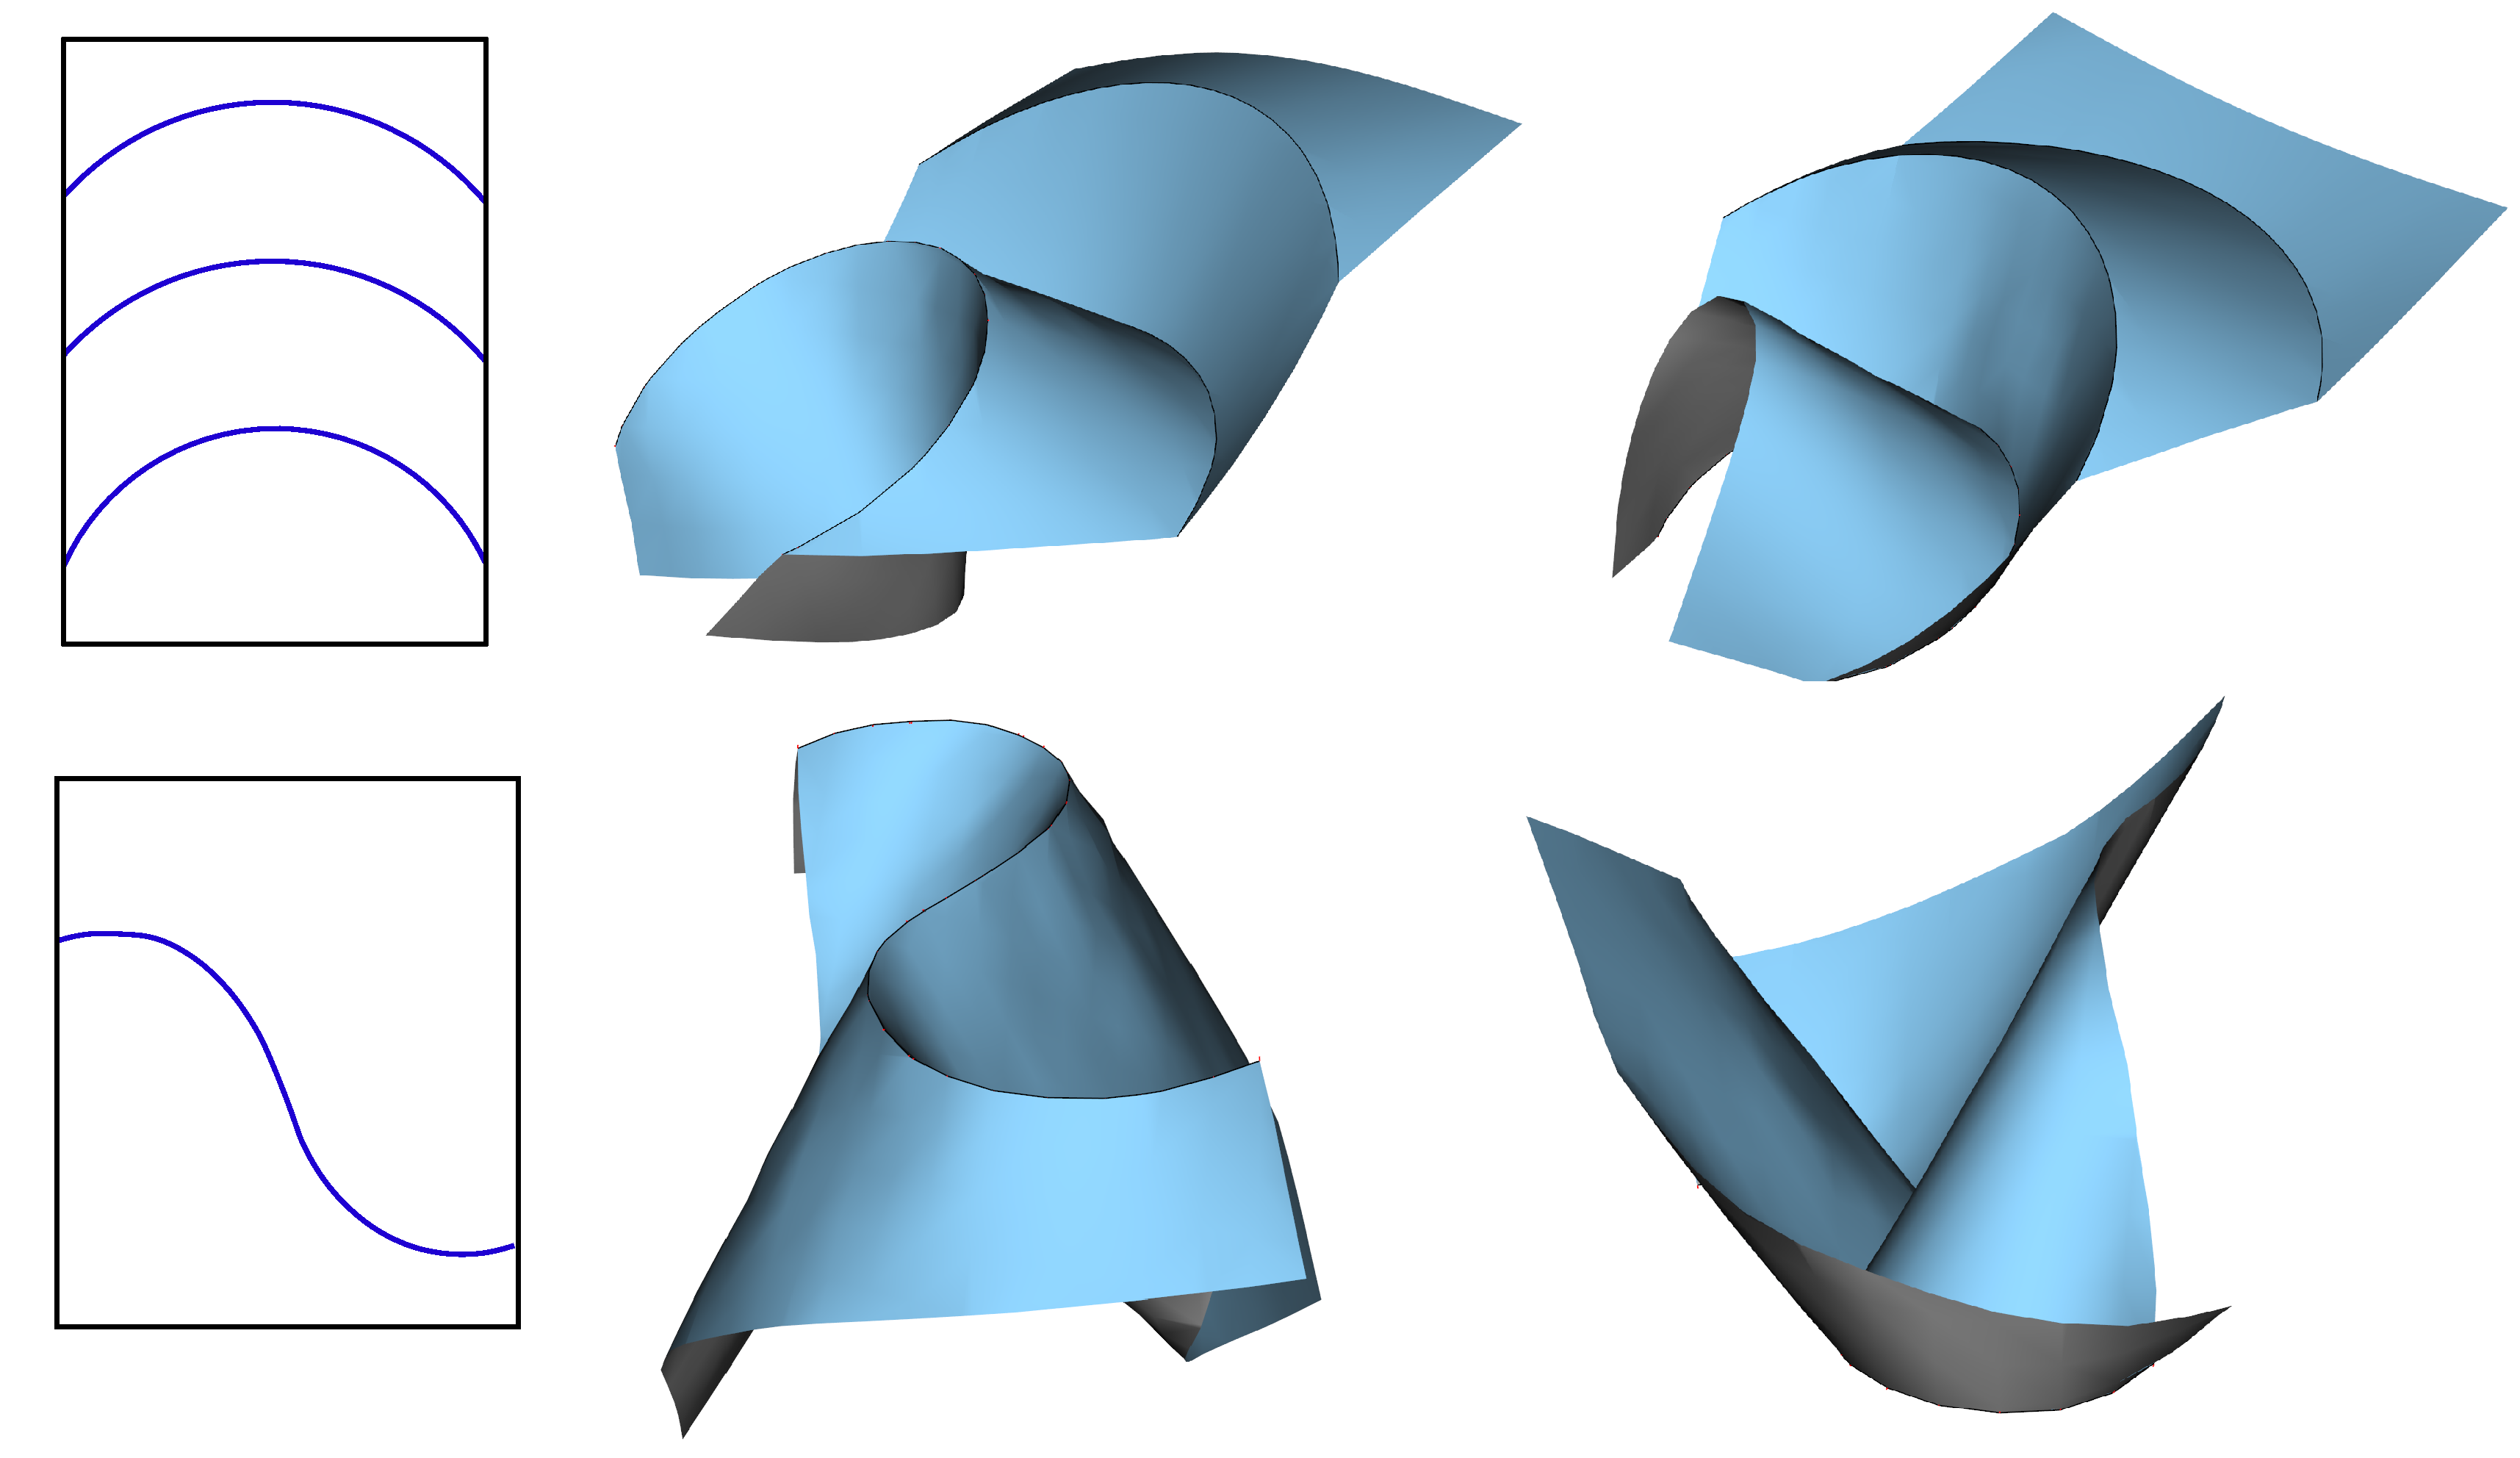
\includegraphics[width=\linewidth]{figures/MV_bias_modeling}
	\caption{\MiR{Same pattern, same curve deformation, different mountain/valley assignment by enforcing constraint \eqref{eq:mountain_valley} along the fold.}}
	\label{fig:MV_bias_modeling}
\end{figure}

\begin{figure} [h]
	\centering
	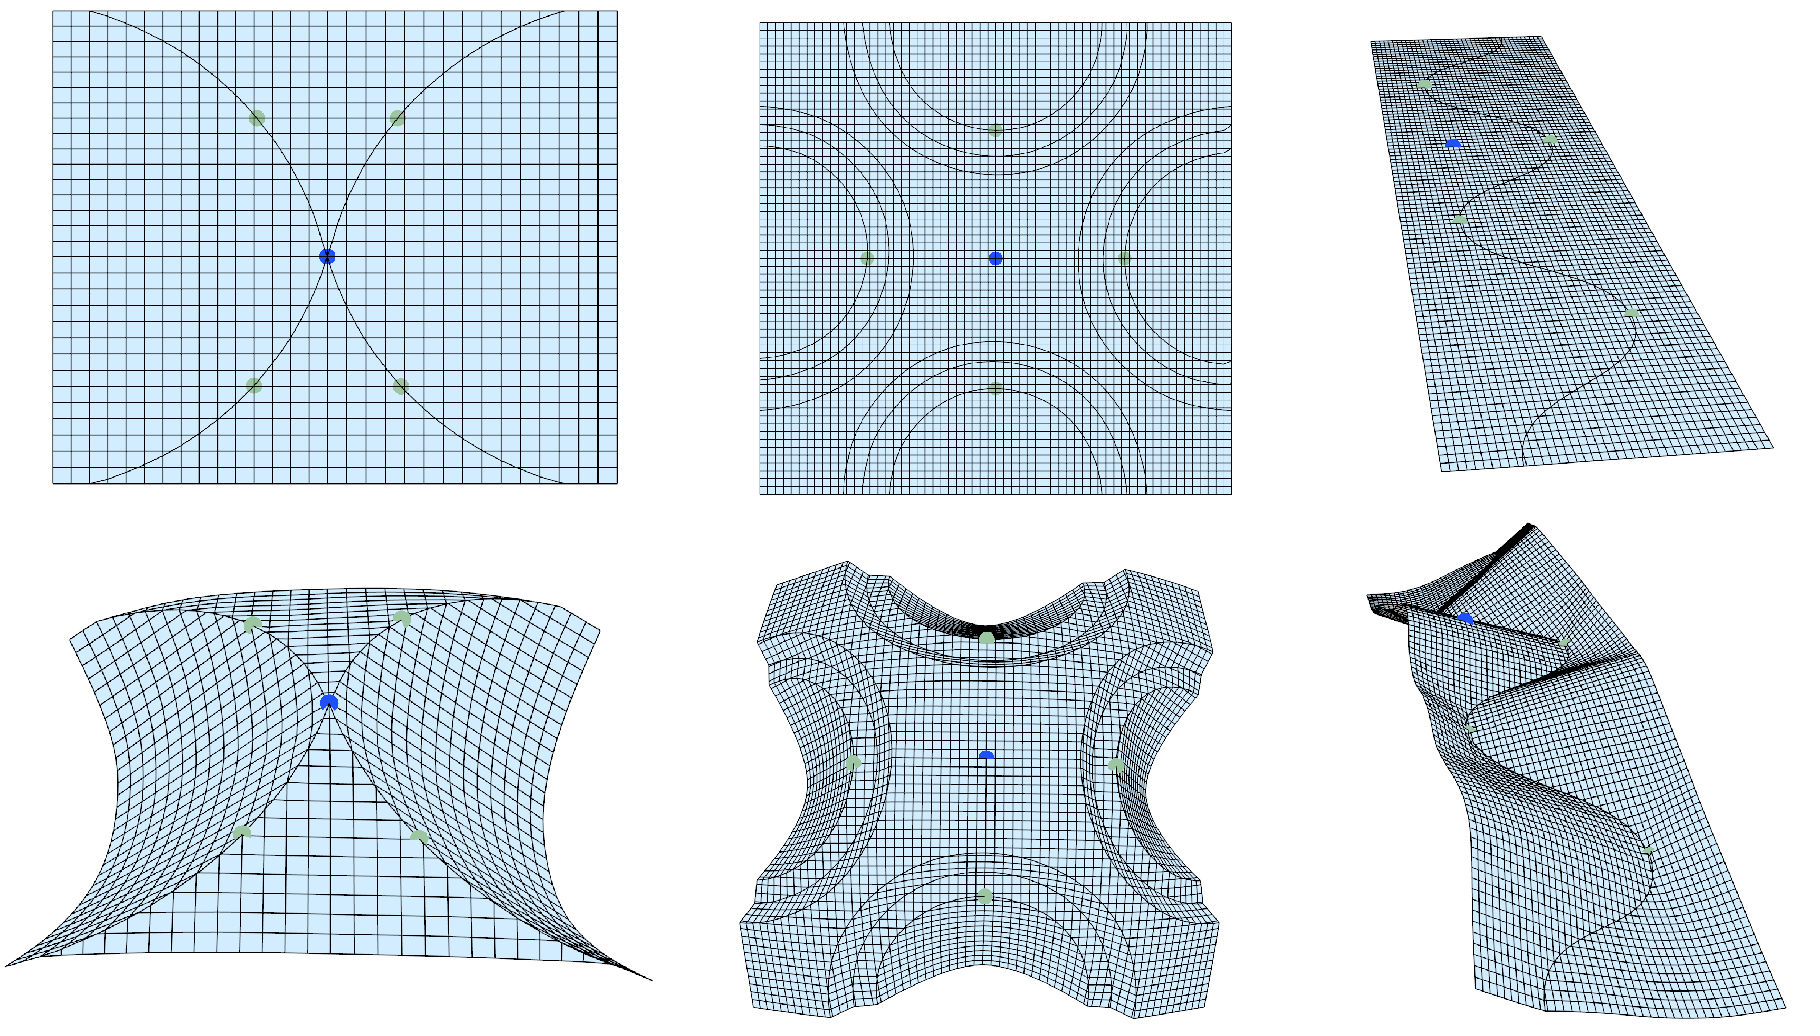
\includegraphics[width=\linewidth]{figures/dihedral_editing}
	\caption{\MiR{A sparse number of dihedral angle constraints(green)  interpolated slowly, with a single positional cosntraint (blue), no M/V assignment was given.}}
	\label{fig:dihedral_editing}
\end{figure}